%%%%%%%%%%%%%%%%%%%%%%%%%%%%%%%%%%%%%%%%%%%%%%%%%%%%%%%%%%%%%%%%%%%%%%%%%%%%%%%%%
%% Documenclass 
%%%%%%%%%%%%%%%%%%%%%%%%%%%%%%%%%%%%%%%%%%%%%%%%%%%%%%%%%%%%%%%%%%%%%%%%%%%%%%%%%
\documentclass[a4paper,oneside,titlepage]{report}
%%%%%%%%%%%%%%%%%%%%%%%%%%%%%%%%%%%%%%%%%%%%%%%%%%%%%%%%%%%%%%%%%%%%%%%%%%%%%%%%%
%% Packages
%%%%%%%%%%%%%%%%%%%%%%%%%%%%%%%%%%%%%%%%%%%%%%%%%%%%%%%%%%%%%%%%%%%%%%%%%%%%%%%%%
\usepackage[english]{babel}
\usepackage{amsmath}
\usepackage{complexity}
\usepackage[T1]{fontenc}
\usepackage[utf8]{inputenc}
\usepackage[pdftex]{graphicx} %%Graphics in pdfLaTeX
\usepackage{a4wide} %%Smaller margins, more text per page.
\usepackage{longtable} %%For tables that exceed a page width
\usepackage{pdflscape} %%Adds PDF sup­port to the land­scape en­vi­ron­ment of pack­age
\usepackage{caption} %%Pro­vides many ways to cus­tomise the cap­tions in float­ing en­vi­ron­ments like fig­ure and ta­ble
\usepackage{float} %%Im­proves the in­ter­face for defin­ing float­ing ob­jects such as fig­ures and ta­bles
\usepackage[tablegrid,nochapter]{vhistory} %%Vhis­tory sim­pli­fies the cre­ation of a his­tory of ver­sions of a doc­u­ment
\usepackage[nottoc]{tocbibind} %%Au­to­mat­i­cally adds the bib­li­og­ra­phy and/or the in­dex and/or the con­tents, etc., to the Ta­ble of Con­tents list­ing
\usepackage[toc,page]{appendix} %%The ap­pendix pack­age pro­vides var­i­ous ways of for­mat­ting the ti­tles of ap­pen­dices
\usepackage{pdfpages} %%This pack­age sim­pli­fies the in­clu­sion of ex­ter­nal multi-page PDF doc­u­ments in LATEX doc­u­ments
\usepackage[rightcaption]{sidecap} %%De­fines en­vi­ron­ments called SC­fig­ure and SCtable (anal­o­gous to fig­ure and ta­ble) to type­set cap­tions side­ways
\usepackage{cite} %%The pack­age sup­ports com­pressed, sorted lists of nu­mer­i­cal ci­ta­tions, and also deals with var­i­ous punc­tu­a­tion and other is­sues of rep­re­sen­ta­tion, in­clud­ing com­pre­hen­sive man­age­ment of break points
\usepackage[]{acronym} %%This pack­age en­sures that all acronyms used in the text are spelled out in full at least once. It also pro­vides an en­vi­ron­ment to build a list of acronyms used
\usepackage[pdftex,scale={.8,.8}]{geometry} %%The pack­age pro­vides an easy and flex­i­ble user in­ter­face to cus­tomize page lay­out, im­ple­ment­ing auto-cen­ter­ing and auto-bal­anc­ing mech­a­nisms so that the users have only to give the least de­scrip­tion for the page lay­out. For ex­am­ple, if you want to set each mar­gin 2cm with­out header space, what you need is just \usep­a­ck­age[mar­gin=2cm,no­head]{ge­om­e­try}.
\usepackage{layout} %%The pack­age de­fines a com­mand \lay­out, which will show a sum­mary of the lay­out of the cur­rent doc­u­ment
\usepackage{subfigure} %%Pro­vides sup­port for the ma­nip­u­la­tion and ref­er­ence of small or ‘sub’ fig­ures and ta­bles within a sin­gle fig­ure or ta­ble en­vi­ron­ment.
\usepackage[toc]{glossaries} %%The glos­saries pack­age sup­ports acronyms and mul­ti­ple glos­saries, and has pro­vi­sion for op­er­a­tion in sev­eral lan­guages (us­ing the fa­cil­i­ties of ei­ther ba­bel or poly­glos­sia).
\usepackage[left,pagewise,modulo]{lineno} %%Adds line num­bers to se­lected para­graphs with ref­er­ence pos­si­ble through the LATEX \ref and \pageref cross ref­er­ence mech­a­nism
\usepackage[pdftex,colorlinks=false,hidelinks,pdfstartview=FitV]{hyperref}%%The hy­per­ref pack­age is used to han­dle cross-ref­er­enc­ing com­mands in LATEX to pro­duce hy­per­text links in the doc­u­ment. 
\usepackage{metainfo}
\usepackage[pagestyles,raggedright]{titlesec}
\usepackage{etoolbox}
\usepackage{%
	array, %%An ex­tended im­ple­men­ta­tion of the ar­ray and tab­u­lar en­vi­ron­ments which ex­tends the op­tions for col­umn for­mats, and pro­vides "pro­grammable" for­mat spec­i­fi­ca­tions
	booktabs, %%The pack­age en­hances the qual­ity of ta­bles in LATEX, pro­vid­ing ex­tra com­mands as well as be­hind-the-scenes op­ti­mi­sa­tion
	dcolumn, %%
	rotating,
	shortvrb,
	units,
	url,
	lastpage,
	longtable,
	lscape,
	qtree,
	skmath,	
}
%%%%%%%%%%%%%%%%%%%%%%%%%%%%%%%%%%%%%%%%%%%%%%%%%%%%%%%%%%%%%%%%%%%%%%%%%%%%%%%%%
%% Java --> latex 
%%%%%%%%%%%%%%%%%%%%%%%%%%%%%%%%%%%%%%%%%%%%%%%%%%%%%%%%%%%%%%%%%%%%%%%%%%%%%%%%%
\usepackage{listings}
\usepackage{color}
\definecolor{pblue}{rgb}{0.13,0.13,1}
\definecolor{pgreen}{rgb}{0,0.5,0}
\definecolor{pred}{rgb}{0.9,0,0}
\definecolor{pgrey}{rgb}{0.46,0.45,0.48}
\usepackage{inconsolata}
%%%%%%%%%%%%%%%%%%%%%%%%%%%%%%%%%%%%%%%%%%%%%%%%%%%%%%%%%%%%%%%%%%%%%%%%%%%%%%%%%
\setlength{\parindent}{0pt}
\setlength{\parskip}{.5\baselineskip}
%%%%%%%%%%%%%%%%%%%%%%%%%%%%%%%%%%%%%%%%%%%%%%%%%%%%%%%%%%%%%%%%%%%%%%%%%%%%%%%%%
%% Inserting the metadata
%%%%%%%%%%%%%%%%%%%%%%%%%%%%%%%%%%%%%%%%%%%%%%%%%%%%%%%%%%%%%%%%%%%%%%%%%%%%%%%%%
% % Metadaten des Dokumentes

\def\Company{Private}
\def\Institute{\textit{University of Pretoria}}
\def\Course{\textit{Software Engineering (COS730)}}
\def\Module{\textit{ }}
\def\Docent{\textit{Ms. Stacey A. Baror}}
\def\Assistant{\textit{}}

\def\BoldTitle{Software Requirements Specification}

\def\Subtitle{for \\ Live Action Role-play facilitating system \\}
\def\Authors{Prepared by:\\\\ Chris A. Pieterse (u12004333) } 
\def\Shortname{A.Sandu}


\title{\textbf{\BoldTitle}\\\Subtitle}
\author{\Authors \\ \\ \\ \Institute\\ \Course\\ \Module\\ \Docent\\ \Assistant}
\date{Pretoria, 12. April 2021}

%%%%%%%%%%%%%%%%%%%%%%%%%%%%%%%%%%%%%%%%%%%%%%%%%%%%%%%%%%%%%%%%%%%%%%%%%%%%%%%%%
%% Creation of pdf information
%%%%%%%%%%%%%%%%%%%%%%%%%%%%%%%%%%%%%%%%%%%%%%%%%%%%%%%%%%%%%%%%%%%%%%%%%%%%%%%%%
\hypersetup{pdfinfo={
		Title={Title},
		Author={TR},
		Subject={Report}
	}}
%%%%%%%%%%%%%%%%%%%%%%%%%%%%%%%%%%%%%%%%%%%%%%%%%%%%%%%%%%%%%%%%%%%%%%%%%%%%%%%%%
%% Creating the frontpage
%%%%%%%%%%%%%%%%%%%%%%%%%%%%%%%%%%%%%%%%%%%%%%%%%%%%%%%%%%%%%%%%%%%%%%%%%%%%%%%%%
\AtBeginDocument{
	\maketitle
	\thispagestyle{empty}
}

%%%%%%%%%%%%%%%%%%%%%%%%%%%%%%%%%%%%%%%%%%%%%%%%%%%%%%%%%%%%%%%%%%%%%%%%%%%%%%%%%
%% Creation of the header
%%%%%%%%%%%%%%%%%%%%%%%%%%%%%%%%%%%%%%%%%%%%%%%%%%%%%%%%%%%%%%%%%%%%%%%%%%%%%%%%%
\patchcmd{\chapter}{plain}{short}{}{} %$ <-- the header on chapter 1
%%%%%%%%%%%%%%%%%%%%%%%%%%%%%%%%%%%%%%%%%%%%%%%%%%%%%%%%%%%%%%%%%%%%%%%%%%%%%%%%%
%% Creation of page-styles
%%%%%%%%%%%%%%%%%%%%%%%%%%%%%%%%%%%%%%%%%%%%%%%%%%%%%%%%%%%%%%%%%%%%%%%%%%%%%%%%%
\newpagestyle{long}{%
	\sethead[\thepage][][\chaptername\ \thechapter:\ \chaptertitle]{\chaptername\ \thechapter:\ \chaptertitle}{}{\thepage}
	\headrule
}

\newpagestyle{short}{%
	\sethead[\thepage][][]{}{}{\thepage}
	\headrule
}
%%%%%%%%%%%%%%%%%%%%%%%%%%%%%%%%%%%%%%%%%%%%%%%%%%%%%%%%%%%%%%%%%%%%%%%%%%%%%%%%%
%% DOCUMENT
%%%%%%%%%%%%%%%%%%%%%%%%%%%%%%%%%%%%%%%%%%%%%%%%%%%%%%%%%%%%%%%%%%%%%%%%%%%%%%%%%
\begin{document}

\pagenumbering{roman}
\DeclareGraphicsExtensions{.pdf,.jpg,.png}
\pagestyle{short}



\newpage
%%%%%%%%%%%%%%%%%%%%%%%%%%%%%%%%%%%%%%%%%%%%%%%%%%%%%%%%%%%%%%%%%%%%%%%%%%%%%%%%%
%% Table of contents
%%%%%%%%%%%%%%%%%%%%%%%%%%%%%%%%%%%%%%%%%%%%%%%%%%%%%%%%%%%%%%%%%%%%%%%%%%%%%%%%%
 \tableofcontents % Inhaltsverzeichnis



\pagestyle{long}




%%%%%%%%%%%%%%%%%%%%%%%%%%%%%%%%%%%%%%%%%%%%%%%%%%%%%%%%%%%%%%%%%%%%%%%%%%%%%%%%%
%% Version table insertion
%%%%%%%%%%%%%%%%%%%%%%%%%%%%%%%%%%%%%%%%%%%%%%%%%%%%%%%%%%%%%%%%%%%%%%%%%%%%%%%%%
%\input{base/history}
\pagenumbering{arabic}
%%%%%%%%%%%%%%%%%%%%%%%%%%%%%%%%%%%%%%%%%%%%%%%%%%%%%%%%%%%%%%%%%%%%%%%%%%%%%%%%%
%% Inserting all the content
%%%%%%%%%%%%%%%%%%%%%%%%%%%%%%%%%%%%%%%%%%%%%%%%%%%%%%%%%%%%%%%%%%%%%%%%%%%%%%%%%
\chapter{Introduction}
\label{ch:intro}
Describe the purpose and scope of the software system- Explain the vision and objectives. State the business need for the application and summarise the scope of the project.

\section{Purpose}
Enhance the immersion of live action role play, and the ease of engagement for new and established participants

\section{Scope}
The facilitation of data transference between implements, users and a centralised information system.

\section{Vision}
Immersive live action role-playing, where participants can free their focus from the “meta-game” and be comfortable that their interaction with other participants are handled consistently and fairly.

\section{Objectives}
\begin{itemize}
\item Handle implement data capturing.
\item Facilitate inter-implement communication.
\item Facilitate implement data transference.
\item Synchronizing data with central information system
\item Synchronizing data between participants
\item Provide information for consumption on centralised information
\end{itemize}


\chapter{User characteristics}
\label{User characteristics}
\section{Participant}
\textbf{Purpose}\newline
To participate in live action role play and engage with other participants.
\newline\newline
\textbf{Educational level} \newline
Rules of engagement
\newline\newline
\textbf{Experience}\newline
Any
\newline\newline
\textbf{Expertise}\newline
Melee Combat
\newline
Ranged Combat
\newline\newline
\textbf{Technical skills}\newline
Technologically literate
\newline\newline

\section{Marshal}
\textbf{Purpose}\newline
To moderate the state of play and enforce rules of engagement.
\newline\newline
\textbf{Educational level} \newline
Formal Rules of engagement
\newline\newline
\textbf{Experience}\newline
Journeyman
\newline\newline
\textbf{Expertise}\newline
Refereeing
\newline
Rules of engagement
\newline\newline
\textbf{Technical skills}\newline
Technologically literate
\newline\newline

\section{Game Master}
\textbf{Purpose}\newline
To moderate and observe the progression of the story and enrich the context of play.
\newline\newline
\textbf{Educational level} \newline
Formal Rules of engagement
\newline\newline
\textbf{Experience}\newline
Master
\newline\newline
\textbf{Expertise}\newline
Melee Combat
\newline
Ranged Combat
\newline\newline
\textbf{Technical skills}\newline
Technologically literate
\newline\newline

\section{Spectator}
\textbf{Purpose}\newline
To observe the state of play, and support their participant, possibly also use the data gathered to formulate some predictions, or gamble on outcomes.
\newline\newline
\textbf{Educational level} \newline
Any
\newline\newline
\textbf{Experience}\newline
Any
\newline\newline
\textbf{Expertise}\newline
Any
\newline\newline
\textbf{Technical skills}\newline
Technologically literate
\newline\newline


\chapter{Functional requirements}
\label{Functional requirements}
\section{Use case diagram}
\subsection{Use  Case 1: Participant Interaction}

\textbf{U1 :} Facilitate interaction between Participant
\begin{figure}[h!]
\centering
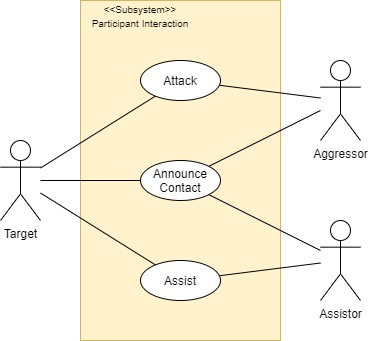
\includegraphics[scale=0.75]{images/ParticipantInteraction.jpg}
\caption{Participant Interaction Subsystem}
\label{fig:ParticipantInteraction}
\end{figure}

\begin{itemize}
\item \textbf{R1 :} Attack
\newline
As an Aggressor, a Participant should be able to attack a Target.
\begin{itemize}
\item \textbf{R1.1 :} Publish damage
\newline
An Aggressor should publish it's damage value to a Target.
\item \textbf{R1.2 :} Handle damage
\newline
A Target should handle incoming damage values from Aggressors, and use defence values to calculate total taken, and health lost.
\end{itemize}
\item \textbf{R2 :} Assist
\newline
As an Assistor, a Participant should be able to assist a Target.
\begin{itemize}
\item \textbf{R2.1 :} Publish aid
\newline
An Assistor should publish it's aid value to a Target.
\item \textbf{R2.2 :} Handle aid
\newline
A Target should handle incoming aid values from Assistors, and calculate health gained.
\end{itemize}
\item \textbf{R3 :} Announce Contact
\newline
As an Target, a Participant should be able to announce contact an Aggressor or Assitor.
\begin{itemize}
\item \textbf{R3.1 :} Publish hit acknowledgement 
\newline
A Target should publish an acknowledgment of contact to Aggressors.
\item \textbf{R3.2 :} Handle hit acknowledgement
\newline
An Aggressor should handle an acknowledgment of contact, and calculate score gained.
\item \textbf{R3.3 :} Publish aid acknowledgement
\newline
A Target should publish an acknowledgment of aid to Assistors.
\item \textbf{R3.4 :} Handle aid acknowledgement
\newline
An Assistors should handle an acknowledgment of aid, and calculate score gained.
\end{itemize}
\end{itemize}

\subsection{Use  Case 2: State of Play Management}
\textbf{U2 :} Managing the State of Play
\begin{figure}[h!]
\centering
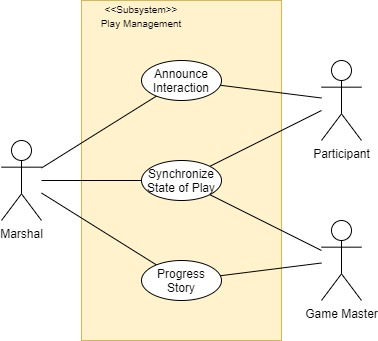
\includegraphics[scale=0.75]{images/EventManagement.jpg}
\caption{Play Management Subsystem}
\label{fig:EventManagement}
\end{figure}

\begin{itemize}
\item \textbf{R4 :} Announce Interaction
\newline
A Participant should be able to Announce Interaction(s) with other Participants.
\begin{itemize}
\item \textbf{R4.1 :} Publish interaction
\newline
A Participant should publish interactions with other Participants to the play log.
\item \textbf{R4.2 :} Handle interaction
\newline
A Marshal should handle interaction announcements and consolidate the state of play for the Participants.
\end{itemize}
\item \textbf{R5 :} Synchronize State of Play 
\newline
A Marshal should be able to Synchronize the State of Play between Participants and the Game Master.
\begin{itemize}
\item \textbf{R5.1 :} Publish event state
\newline
A Marshal should publish the state of play to all Participants and the Game Master.
\item \textbf{R5.2 :} Handle event state
\newline
A Participant should handle state of play updates and adjust it's state and the context they find themselves in accordingly.
\newline
A Game Master should handle state of play updates and adjust the world state and context accordingly.
\end{itemize}
\item \textbf{R6 :} Progress Story
\newline
A Game Master should be able to Progress the Story of the play through the Marshal.
\begin{itemize}
\item \textbf{R6.1 :} Publish world event 
\newline
A Game Master should publish world events, meant to progress the story, to the play log.
\item \textbf{R6.2 :} Handle world event
\newline
A Marshal should handle world event updates and consolidate the state of play for the Participants.
\end{itemize}
\end{itemize}

\subsection{Use  Case 3: Community Engagement}
\textbf{U3 :} Facilitate Engagement with Community
\begin{figure}[h!]
\centering
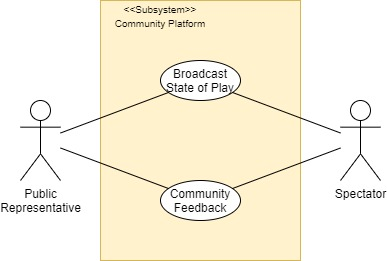
\includegraphics[scale=0.75]{images/CommunityEngagement.jpg}
\caption{Community Platform Subsystem}
\label{fig:CommunityEngagement}
\end{figure}

\begin{itemize}
\item \textbf{R7 :} Broadcast State of play 
\newline
A Public Representative should be able to broadcast the World/Play State for Spectator consumption.
\begin{itemize}
\item \textbf{R1.1 :} Publish world state
\newline
A Public Representative should publish the world state periodically, or on request.
\item \textbf{R1.2 :} Handle world state
\newline
A Spectator should handle world state updates and take it into consideration when providing feedback.
\end{itemize}
\item \textbf{R8 :} Community feedback
\newline
A Spectator should be able to provide Feedback for community consideration.
\begin{itemize}
\item \textbf{R2.1 :} Publish feedback
\newline
A Spectator should publish feedback on the world state.
\item \textbf{R2.2 :} Handle feedback
\newline
A Public Representative should handle the feedback and take it into consideration when generating world events.
\end{itemize}
\end{itemize}

\section{Traceability matrix}
\begin{tabular}{ |p{2cm}||p{4.5cm}|p{4cm}|p{4.5cm}|  }
 \hline
 Requirements & Participant Interaction (U1) & Play Management (U2) & Community Platform (U3) \\
 \hline
 \centering R1 & R1.1, R1.2 & - & - \\
 \centering R2 & R2.1, R2.2 & - & - \\
 \centering R3 & R3.1, R3.2, R3.3, R3.4 & - & - \\
 \centering R4 & - & R4.1, R4.2 & - \\
 \centering R5 & - & R5.1, R5.2 & - \\
 \centering R6 & - & R6.1, R6.2 & - \\
 \centering R7 & - & - & R7.1, R7.2\\
 \centering R8 & - & - & R8.1, R8.2\\
 \hline
\end{tabular}


\chapter{Domain models}
\label{Domain models}
\section{Domain model class diagrams}

\begin{figure}[h!]
\centering
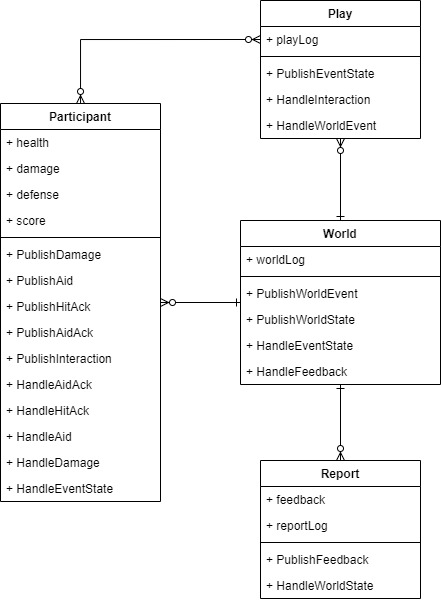
\includegraphics[scale=0.5]{images/CompleteDomainModelClassDiagram.jpg}
\caption{Complete Domain Model Class Diagram}
\label{fig:CompleteDomainModelClassDiagram}
\end{figure}

\textbf{Participant}
\newline
The Participant, as it appears in Figure \ref{fig:CompleteDomainModelClassDiagram}. is composed from the properties:
\begin{itemize}
\item \textbf{health} - Used to determine whether a participant is alive or deceased, and by extension whether they can interact with the play. 
\item \textbf{damage} - Used to determine the value of damage a participant publishes to targeted participant.
\item \textbf{defence} - Used to determine how much health a participant loses from incoming damage.
\item \textbf{score} - Used to determine whether a participant succeeding in the play.
\end{itemize}
Participants must belong to a world, but does not necessarily need to participate in play(s).
\newline

\textbf{Play}
\newline
The Play, as it appears in Figure \ref{fig:CompleteDomainModelClassDiagram}. is composed from the properties:
\begin{itemize}
\item \textbf{play log} - Used to determine the state of play, and the interactions between participants, the play environment, and the greater world.
\end{itemize}
A Play must belong to a world, and contain at least one participant.
\newline

\textbf{World}
\newline
The World, as it appears in Figure \ref{fig:CompleteDomainModelClassDiagram}. is composed from the properties:
\begin{itemize}
\item \textbf{world log} - Used to determine the state of the world, and the events that contribute to the world context.
\end{itemize}
A World is required by all other domain models.
\newline

\textbf{Report}
\newline
The Report, as it appears in Figure \ref{fig:CompleteDomainModelClassDiagram}. is composed from the properties:
\begin{itemize}
\item \textbf{feedback} - Used to determine community opinion about the state of the world. 
\item \textbf{report log} - the state of the world, reduced to fulfill the interests of the report.
\end{itemize}
A Report must belong to a world.
\newline


\section{System Sequence diagrams}
\textbf{Participant Interaction}
\newline
Participant interaction, as depicted in Figure \ref{fig:ParticipantInteractionSequenceDiagram}.
\begin{itemize}
\item \textbf{(a) Aggressor sequence} - The Aggressor participant interacts with a Target participant, and notifies the system about the interaction.
   \begin{itemize}
     \item Publishes damage to Target
     \item Handles contact acknowledgement from Target
     \item Publishes interaction to system
     \item Handles play state update from system
   \end{itemize}
\item \textbf{(b) Assistor sequence} - The Assistor participant interacts with a Target participant, and notifies the system about the interaction.
   \begin{itemize}
     \item Publishes aid to Target
     \item Handles aid acknowledgement from Target
     \item Publishes interaction to system
     \item Handles play state update from system
   \end{itemize}
\item \textbf{(c) Target sequence} - The Target participant interacts with a Aggressor/Assistor participant, and notifies the system about the interaction.
   \begin{itemize}
     \item Publishes contact acknowledgement to Aggressor
     \item Handles damage from Aggressor
     \item Publishes aid acknowledgement to Assistor
     \item Handles aid from Assistor
     \item Publishes interaction to system
     \item Handles play state update from system
   \end{itemize}
\end{itemize}
\begin{figure}[H]
\centering
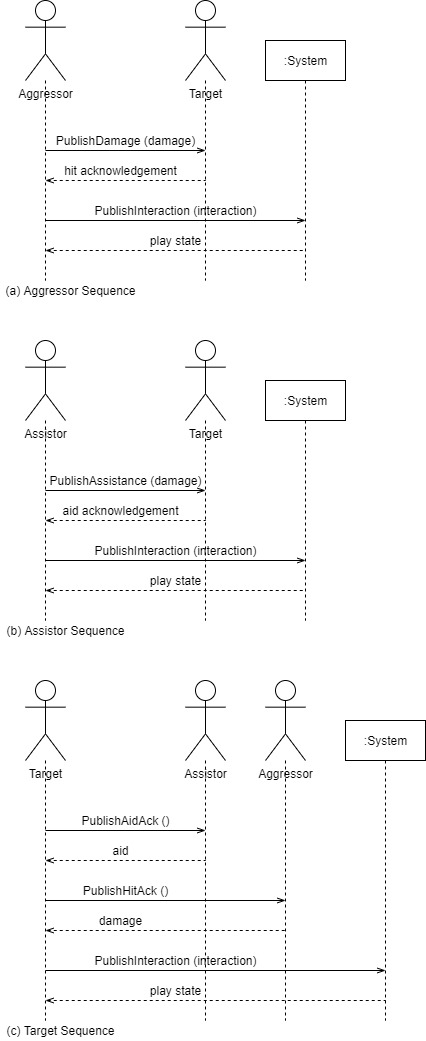
\includegraphics[scale=0.5]{images/ParticipantInteractionSequenceDiagram .jpg}
\caption{Participant Interaction System Sequence Diagram (a) Aggressor sequence (b) Assistor sequence (c) Target sequence}
\label{fig:ParticipantInteractionSequenceDiagram}
\end{figure}

\textbf{Play Management}
\newline
Play management, as depicted in Figure \ref{fig:PlayManagementSequenceDiagram}.
\begin{itemize}
\item \textbf{(a) Marshal sequence} - The Marshal consolidates the participant interactions and world events into a synchronised, consistent play state.
   \begin{itemize}
     \item Publishes state of play to system, for distribution to Participants and the Game master
     \item Handles interaction announcements from the system, and consolidates them to the play log
     \item Handles world events from the system, and consolidates them to the play log
   \end{itemize}
\item \textbf{(b) Game master sequence} - The Game master consolidates the play states into the world state, and steers the play state with world events.
   \begin{itemize}
     \item Publishes a world event to the system, to steer state of play
     \item Handles play state updates from the system, and consolidates them into the world log
   \end{itemize}
\end{itemize}
\begin{figure}[H]
\centering
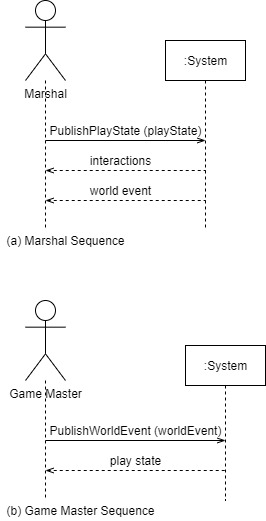
\includegraphics[scale=0.5]{images/PlayManagementSequenceDiagram.jpg}
\caption{Play Management Sequence Diagram (a) Marshal sequence (b) Game master sequence}
\label{fig:PlayManagementSequenceDiagram}
\end{figure}

\textbf{Community Engagement}
\newline
Community engagement, as depicted in Figure \ref{fig:CommunityEngagementSequenceDiagram}.
\begin{itemize}
\item \textbf{Community engagement sequence} - The Spectator consumes world states and provides feedback on the community's opinion of the state of the world.
   \begin{itemize}
     \item Publishes feedback to the system
     \item Handles world state updates, and determines the opinion of the community for progress of world state 
   \end{itemize}
\end{itemize}
\begin{figure}[H]
\centering
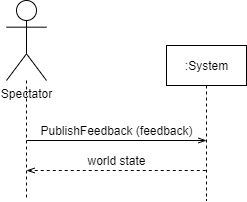
\includegraphics[scale=0.5]{images/CommunityEngagementSequenceDiagram.jpg}
\caption{Community Engagement Sequence Diagram}
\label{fig:CommunityEngagementSequenceDiagram}
\end{figure}


\chapter{Non-functional requirements}
\label{Functional requirements}
\section{Quality requirements}
\begin{itemize}
\item \textbf{Performance}
    \newline
    The system will be distributed over:
    \begin{itemize}
        \item Embedded systems
        \item Mobile systems
        \item cloud hosted systems
    \end{itemize}
    and should perform real-time computations, therefore it should be optimised on each respective system.
    \newline
\item \textbf{Reliability}
    \newline
    The system will be operating in real time, and the course of play, and user experience will be greatly impacted by reliability issues.
    \newline
\item \textbf{Security}
    \newline
    The system should make use of basic authentication, but no personal information about the users will be persisted, thus removing the risk of personal data leaks.
    \newline
\item \textbf{Maintainability}
    \newline
    The system should comply to modern best practices, and sufficient domain abstraction, to improve comprehension by industry professionals.
    \newline
\item \textbf{Useability}
    \newline
    The system should facilitate the play, and as such user interaction with the system should be implicit through user actions.
    \newline
\item \textbf{Flexibility}
    \newline
    The system should be open for OEM's to extend the functionality of the system in new and intuitive ways that will enhance the user experience.
    \newline
\end{itemize}
\pagebreak

\section{Specify and quantify}
\begin{itemize}
\item \textbf{Performance}
    \begin{itemize}
        \item Embedded systems: Handle simultaneous interactions.
        \item Mobile systems: No more than a 10\% footprint on mobile battery.
        \item cloud hosted systems: Support up to 50 simultaneous users.
    \end{itemize}
\item \textbf{Reliability}
    \newline
    In the case that any of the systems should fail, the rest of the systems should be unaffected.
    \newline
\item \textbf{Security}
    \newline
    The system should make use of basic authentication.
    The system should not persist personal information about the users.
    \newline
\item \textbf{Maintainability}
    \begin{itemize}
        \item S.O.L.I.D. Principal compliant software architecture.
        \item TDD implementation approach.
    \end{itemize}
\item \textbf{Useability}
    \newline
    The system should limit user goal fulfillment steps to a maximum of 3.
    \newline
\end{itemize}




%%%%%%%%%%%%%%%%%%%%%%%%%%%%%%%%%%%%%%%%%%%%%%%%%%%%%%%%%%%%%%%%%%%%%%%%%%%%%%%%%
%% Source defintions
%%%%%%%%%%%%%%%%%%%%%%%%%%%%%%%%%%%%%%%%%%%%%%%%%%%%%%%%%%%%%%%%%%%%%%%%%%%%%%%%%
% When no use outcomment
%\include{base/sources}
%%%%%%%%%%%%%%%%%%%%%%%%%%%%%%%%%%%%%%%%%%%%%%%%%%%%%%%%%%%%%%%%%%%%%%%%%%%%%%%%%
%% Inserting the appendix
%%%%%%%%%%%%%%%%%%%%%%%%%%%%%%%%%%%%%%%%%%%%%%%%%%%%%%%%%%%%%%%%%%%%%%%%%%%%%%%%%
% When no use outcomment
%\include{appendix/appendix}
\end{document}*/***********************************************************************8	
